\section{Latent variable models}

The philosophy behind latent variable models is that we have \textit{observables} $\vec{X}$, which
are augmented by \textit{latent variables} $\vec{Z}$, which happens by specifying a
\textit{complete data model} $p(\vec{X}, \vec{Z})$, which implies a \textit{marginal model}, \[
    p(\vec{X} = \vec{x}) = \sum_{\vec{z} \in \mathcal{Z}} p(\vec{X} = \vec{x}, \vec{Z} = \vec{z}).
\]
The marginal model can be specified by a conditional $p(\mat{X} \mid \mat{Z})$ and prior
$p(\mat{Z})$, \[
    p(\vec{X} = \vec{x}) = \sum_{\vec{z} \in \mathcal{Z}} p(\vec{X} = \vec{x} \mid \vec{Z} = \vec{z}) p(\vec{Z} = \vec{z}).
\]

\subsection{Probabilistic clustering models}

Assume we are given a dataset of $s$ observables $\{ \vec{x}_t \mid t \in [s] \}$. The conceptually
simplest family of latent variable models assigns a $k$-class categorical random variable $Z_t$ to
each observable. The latent information tags an observable as a member of that class.

Specifically, we have the following prior categorical distribution, \[
    Z_t \sim \mathrm{Categorical}(\pi_1, \ldots, \pi_k), \quad P(Z_t = z) = \pi_z,
\]
where $\vec{\pi} \in \Delta^{k-1}$ is an unknown parameter.\sidenote{$\Delta^{k-1}$ is the
    $k$-dimensional probability simplex, which is the space of vectors where all elements are
    non-negative and sum to 1.} To fully parametrize the latent variable model, we need a class
conditional distribution for each class, $p(\vec{x} \mid z)$. By parametrizing the
class-conditional distribution of $z$ by $\vec{\theta}_z$, we have the following parametrized
distribution over $\vec{X}$, \[
    p(\vec{x}; \vec{\theta}) = \sum_{z=1}^{k} p(z) p(\vec{x} \mid z) = \sum_{z=1}^{k} \pi_z p(\vec{x}; \vec{\theta}_z).
\]
We interpret this as a mixture distribution; convex combinations of class-specific distributions.
Moreover, this model is fully parametrized by the prior and class-conditional distribution
parameters, \[
    \vec{\theta} = [\vec{\pi}, \vec{\theta}_1, \ldots, \vec{\theta}_k].
\]
For given parameters $\vec{\theta}$, we can use Bayes' rule to compute the latent posteriors, \[
    p(z \mid \vec{x}; \vec{\theta}) = \frac{\pi_z p(\vec{x}; \vec{\theta}_z)}{\sum_{\zeta=1}^{k} \pi_{\zeta} p(\vec{x}; \vec{\theta}_{\zeta})}.
\]
We can interpret these probabilities as observable-specific probabilistic cluster memberships.

\paragraph{Learning the parameters.}

A common approach to learn the best parameters is to maximize the likelihood of the data, which is
called maximum likelihood estimation (MLE). In other words, we choose the model parameters that
maximize the probability of the observed data, \[
    \ell(\vec{\theta}; \{ \vec{x}_1, \ldots, \vec{x}_s \}) = \sum_{t=1}^{s} \log p(\vec{x}_t; \vec{\theta}) = \sum_{t=1}^{s} \log \sum_{z=1}^{k} \pi_z p(\vec{x}_t; \vec{\theta}_z). \margintag{We take the log-likelihood for improved numerical stability.}
\]
This gives us the following optimization problem, \[
    \vec{\theta}^{\mathrm{MLE}} \in \argmax_{\vec{\theta}} \ell(\vec{\theta}; \{ \vec{x}_1, \ldots, \vec{x}_s \}),
\]
which we optimize by the expectation-maximization (EM) algorithm. The EM algorithm is a general
tool for learning in latent variable models, but we will introduce it in the context of mixture
models.

Let $\vec{q}_t \in \Delta^{k-1}, \forall t \in [s]$ be the variational parameters. Using this we
can derive the evidence lower bound (ELBO),
\begin{align*}
    \ell(\vec{\theta}; \{ \vec{x}_1, \ldots, \vec{x}_s \}) & = \sum_{t=1}^{s} \log \sum_{z=1}^{k} q_{tz} \frac{\pi_z}{q_{tz}} p(\vec{x}; \vec{\theta}_z)                                                 \\
                                                           & \geq \sum_{t=1}^{s} \sum_{z=1}^{k} q_{tz} \log \lft( \frac{\pi_z}{q_{tz}} p(\vec{x}; \vec{\theta}_z) \rgt) \margintag{Jensen's inequality.} \\
                                                           & = \sum_{t=1}^{s} \sum_{z=1}^{k} q_{tz} \log p(\vec{x}; \vec{\theta}_z) - \sum_{z=1}^{k} q_{tz} \log \frac{q_{tz}}{\pi_z}                    \\
                                                           & = \sum_{t=1}^{s} \sum_{z=1}^{k} q_{tz} \log p(\vec{x}; \vec{\theta}_z) - D_{\mathrm{KL}}(\vec{q}_t \| \vec{\pi}).
\end{align*}
Since this lower bounds the MLE, we can use the ELBO as an objective to implicitly maximize the log-likelihood. Maximizing \wrt
$\vec{q}$ increases the tightness of the bound of ELBO on the MLE,\sidenote{$\vec{q}$ does not affect
    the likelihood, so an increase can only tighten the bound.} while maximizing \wrt $\vec{\theta}$
improves the model fit.

Firstly, we will solve for the optimal choice of $\vec{q}_t$, \[
    \sum_{t=1}^{s} \sum_{z=1}^{k} q_{tz} \log p(\vec{x}; \vec{\theta}_z) - D_{\mathrm{KL}}(\vec{q}_t \| \vec{\pi}), \quad \sum_{z=1}^{k} q_{tz} = 1, \forall t \in [s].
\]
We can solve for every $\vec{q}_t$ independently, because the ELBO is separable \wrt $\vec{q}_t$.
Furthermore, we enforce the normalization constraint on $\vec{q}$ by introducing a Lagrange
multiplier $\lambda$. This results in the following objective to maximize per $\vec{q}_t$, \[
    \vec{q}_t^\star \in \argmax_{\vec{q}_t} \ell(\vec{q}_t) \doteq \sum_{z=1}^{k} q_{tz} \lft( \log p(\vec{x}_t; \vec{\theta}_z) - \log \frac{q_{tz}}{\pi_z} \rgt) - \lambda \lft( \sum_{z=1}^{k} q_{tz} - 1 \rgt).
\]
The derivative \wrt $q_{tz}$ of this function is
\begin{align*}
    \pdv{\ell(\vec{q}_t)}{q_{tz}} & = \pdv*{\sum_{z'=1}^{k} q_{tz'} \lft( \log p(\vec{x}_t; \vec{\theta}_{z'}) + \log \pi_{z'} - \log q_{tz'} \rgt)}{q_{tz}} \\
                                  & = \log p(\vec{x}_t; \vec{\theta}_z) + \log \pi_z - \pdv*{q_{tz} \log q_{tz}}{q_{tz}} - \lambda                           \\
                                  & = \log p(\vec{x}_t; \vec{\theta}_z) + \log \pi_z - \log q_{tz} - \frac{q_{tz}}{q_{tz}} - \lambda                         \\
                                  & = \log p(\vec{x}_t; \vec{\theta}_z) + \log \pi_z - \log q_{tz} - \lambda - 1.
\end{align*}
Thus, we have the following first-order optimality condition, \[
    \log p(\vec{x}_t; \vec{\theta}_z) + \log \pi_z - \log q_{tz} \overset{!}{=} \lambda + 1.
\]
Exponentiating both sides yields \[
    q_{tz} \overset{!}{=} \frac{\pi_z p(\vec{x}_t; \vec{\theta}_z)}{e^{\lambda+1}}.
\]
Enforcing the constraint of $\vec{q}_t \in \Delta^{k-1}$, we get \[
    q_{tz} = \frac{\pi_z p(\vec{x}_t; \vec{\theta}_z)}{\sum_{\zeta=1}^{k} \pi_{\zeta}p(\vec{x}_t; \vec{\theta}_{\zeta})}.
\]
As we saw before, this is the posterior of the latent class variable $p(z \mid \vec{x}_t;
    \vec{\theta})$. Note that the optimal choice of the variational parameters $\vec{q}_t$ depends on
the parameters $\vec{\theta}$. Hence, it is only a partial step, called the expectation (E) step.

Now we also need a step to maximize the model parameters $\vec{\theta}$. We can easily solve for
$\vec{\pi}$ by \[
    \pi^{\star}_z = p(z) = \sum_{t=1}^{s} p(\vec{x}_t, z) = \sum_{t=1}^{s} p(z \mid \vec{x}_t \mid z) p(z) = \frac{1}{s} \sum_{t=1}^{s} q_{tz}. \margintag{This assumes that the data are distributed uniformly. It can also be derived by the first-order optimality condition.}
\]
Moreover, the solution for $\vec{\theta}_z$ depends on the choice of the model distribution, but we
can generally get to separable problems, \[
    \vec{\theta}^{\star}_z \in \argmax_{\vec{\theta}_z} \sum_{t=1}^{s} q_{tz} \log p(\vec{x}_t; \vec{\theta}_z).
\]
This means that the parameters for different classes $z$ are decoupled given the variational
parameters $\vec{q}$. Thus, for each component, we only have to solve a weighted MLE problem, which
is often possible to do analytically. This partial step is called the maximization (M) step.

\paragraph{Gaussian mixture model.}

We will consider a common special case of the above framework, where we specify the component
models $p(\vec{X} \mid Z)$ by Gaussians with unit variance, \[
    p(\vec{x}; \vec{\pi}, \{ \vec{\mu}_1, \ldots, \vec{\mu}_k \}) = \sum_{z=1}^{k} \pi_z \mathcal{N}(\vec{x}; \vec{\mu}_z, \mat{I}),
\]
where \[
    \mathcal{N}(\vec{x}; \vec{\mu}, \mat{\Sigma}) = (2\pi)^{-\nicefrac{d}{2}} \det{\mat{\Sigma}}^{-\nicefrac{1}{2}} \exp \lft( -\frac{1}{2} \transpose{(\vec{x} - \vec{\mu})} \mat{\Sigma}^{-1} (\vec{x} - \vec{\mu}) \rgt).
\]
The EM algorithm then consists of the following alternating equations,
\begin{gather*}
    q_{tz} \doteq p(z \mid \vec{x}_t, \vec{\theta}) = \frac{\pi_z \exp \lft( -\frac{1}{2} \| \vec{z}_t - \vec{\mu_z} \|^2 \rgt)}{\sum_{\zeta=1}^{k} \pi_{\zeta} \exp \lft( -\frac{1}{2} \| \vec{z}_t - \vec{\mu}_{\zeta} \|^2 \rgt)} \margintag{E-step.} \\
    \vec{\mu}_z = \frac{\sum_{t=1}^{s} q_{tz} \vec{x}_t}{\sum_{t=1}^{s} q_{tz}}, \quad \pi_z = \frac{1}{s} \sum_{t=1}^{s} q_{tz}. \margintag{M-step.}
\end{gather*}
Intuitively, the E-step (soft) clusters the data points and the M-step computes the weighted centroids of each component.

\subsection{Topic models}

We will now consider a class of latent variable models known as topic models. These are used to
analyze document collections and to discover the topical content of documents. Informally, topical
content is the information that the words of a document carry about what the document is about.

Let $\Sigma$ be the word vocabulary with $|\Sigma|=m$ words. A document $d_i$ of length $s_i$ is
part of a collection of $n$ documents and is a field of random variables $X_{it}$, whose
realizations are words $x_{it} \in \Sigma, \forall t \in [s_i]$. We will assume that topical
content is invariant to word order.\sidenote{This is known as \textit{exchangeability}, which says
    that the distribution of a sequence of random variables does not change under any permutation of
    their order.} As a consequence, the sufficient statistics of a document are the frequencies of word
occurrences within it. Hence, we can reduce the data to a bag-of-words representation of occurrence
counts, \[
    N_{ij} = | \{ x_{it} = w_j \mid t \in [s_i] \} |.
\]
In words, $N_{ij}$ denotes how often word $w_j$ occurred in document $d_i$. We can thus summarize
the full document corpus in an occurrence matrix, \[
    \mat{N} = [N_{ij}] \in \mathbb{N}^{n \times m}.
\]

Moreover, we have to conceptualize what we mean by ``topic''. Generally, topics refer to things
that people are interested to talk or write about. Hence, we can represent topics by latent
variables $Z \in [k]$, akin to what we saw in mixture models. We will then associate these topics
with word occurrences, which induce topics of entire documents.\sidenote{If we were to associate
    the topic variables with documents, we would effectively be performing document clustering.
    However, in this case, we want the topics of documents to be induced by the words that they
    contain.} Note that topics are not mutually exclusive, since documents can concern multiple.

We will assume that the documents in the corpus were created according to the following generative
process.\sidenote{This is important so we can infer/reverse engineer a model from it. Also, it is
    important to make assumptions about the data explicit.} For each word, we sample a topic from $p(z
    \mid d)$, and then sample the words from $p(w \mid z)$. Thus, in order to define the latent
variable data model, we need a document-conditional distribution over latent variables, $p(z \mid
    d)$, and a topic-conditional distribution over words, $p(w \mid z)$. We can then define a
document-conditional word distribution, \[
    p(w \mid d) = \sum_{z=1}^{k} p(w \mid z) p(z \mid d).
\]
From this, we define the log-likelihood objective as \[
    \ell(\vec{\theta}; \mat{N}) = \log p(\mat{N}; \vec{\theta}) = \sum_{i=1}^{n} \sum_{j=1}^{m} N_{ij} \log p(w_j \mid d_i).
\]

\paragraph{Learning.}

We can equivalently write the log-likelihood objective in terms of the raw data, \[
    \ell(\vec{\theta}) = \sum_{i=1}^{n} \sum_{t=1}^{s_i} \log \sum_{z=1}^{k} p(x_{it} \mid z) p(z \mid d_i).
\]
Similarly to the mixture models, we define an ELBO, \[
    \ell(\vec{\theta}) \geq \sum_{i=1}^{n} \sum_{t=1}^{s_i} \sum_{z=1}^{k} q_{itz} \lft( \log p(x_{it} \mid z) + \log p(z \mid d_i) - \log q_{itz} \rgt).
\]
Moreover, following the same steps, we can derive the EM equations,
\begin{gather*}
    q_{itz} = \frac{p(x_{it} \mid z) p(z \mid d_i)}{\sum_{\zeta=1}^{k} p(x_{it} \mid \zeta) p(\zeta \mid d_i)} \margintag{E-step.} \\
    p(w_j \mid z) = \frac{\sum_{i=1}^{n} \sum_{t=1}^{s_i} q_{itz} \cdot \mathbb{1}\{ x_{it} = w_j \}}{\sum_{i=1}^{n} \sum_{t=1}^{s_i} q_{itz}}, \quad p(z \mid d_i) = \frac{1}{s_i} \sum_{t=1}^{s_i} q_{itz}. \margintag{M-step.}
\end{gather*}
Intuitively, the E-step computes the posterior probabilities, $q_{itz} = p(z \mid x_{it}, d_i)$, where
$p(z \mid d_i)$ acts as a prior. This yields a probabilistic clustering of word occurrences. The
M-step computes the MLE for a $\vec{q}$-weighted multinomial sample. This algorithm will converge,
but not necessarily to the global maximizer.

\begin{important}
    We can use the class-conditional word distribution, $p(w \mid z)$, to find similar
    words that are connected by a common topic.
\end{important}

\paragraph{Latent Dirichlet allocation.}

The problem with the above topic model is that it assumes a fixed set of documents and selects the
parameters to maximize the predictability of words within these. The natural next step is to extend
the above in a way that accounts for modeling unseen documents. The generative process of this
model is that we first choose a distribution over topics, $p(z\mid \vec{\alpha})$. Then, for each
word, sample a topic from $p(z \mid \vec{\alpha})$ and sample the word from $p(w \mid z)$.

Effectively, the latent Dirichlet allocation (LDA) model takes a ``Bayesian step up'' from latent
variable modeling. Its main idea is that it defines a distribution over mixture vectors, \[
    \vec{v} \in \Delta^{k-1},
\]
as a prior over topics. This parameter is distributed according to a Dirichlet distribution, and
has hyperparameter $\vec{\alpha}$, \[
    p(\vec{v}; \vec{\alpha}) \propto \prod_{z=1}^{k} v_z^{\alpha_z - 1}, \quad \alpha_z > 0, \forall z \in [k].
\]
The Dirichlet distribution is chosen as the prior because it is a conjugate prior of the
categorical distribution. Typically, we set $\alpha_k = \alpha$ and optimize $\alpha$ on held-out
validation data.

Let $\mat{U} = [p(w_j \mid z)] \in [0,1]^{m \times k}$, then we have the following distribution,
\begin{align*}
    p(\mat{X}=[x_1, \ldots, x_s] \mid \mat{U}) & = \int \prod_{t=1}^{s} p(x_t \mid \mat{U}, \vec{v}) p(\vec{v}; \vec{\alpha}) \mathrm{d}\vec{v} \\
    p(w_j \mid \mat{U}, \vec{v})               & = \sum_{z=1}^{k} u_{jz} v_z.
\end{align*}
As can be seen, the probabilities are not conditioned on the observed documents. As a result, when a
new document is introduced, we can use the same distributions, whose parameters were learned from an
existing document collection. In this sense, the LDA model is more robust than the topic model that
was initially introduced.

\paragraph{Probabilistic matrix decomposition.}

\begin{marginfigure}
    \centering
    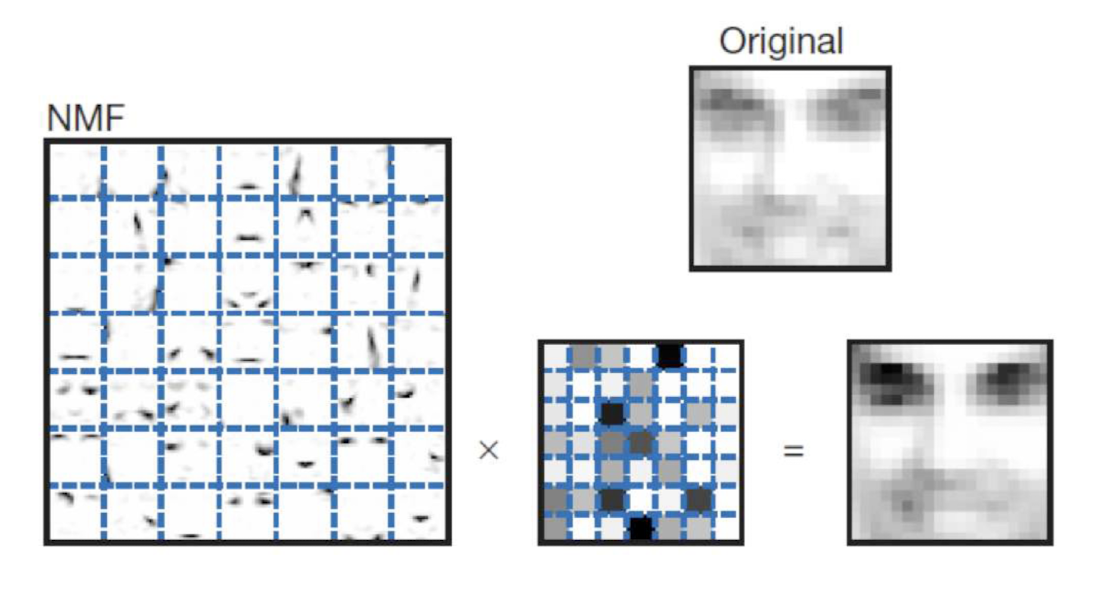
\includegraphics[width=\textwidth]{figures/nmf_face}
    \caption{Factors identified by non-negative matrix factorization in a face reconstruction task.}
    \label{fig:nmf}
\end{marginfigure}

\begin{marginfigure}
    \centering
    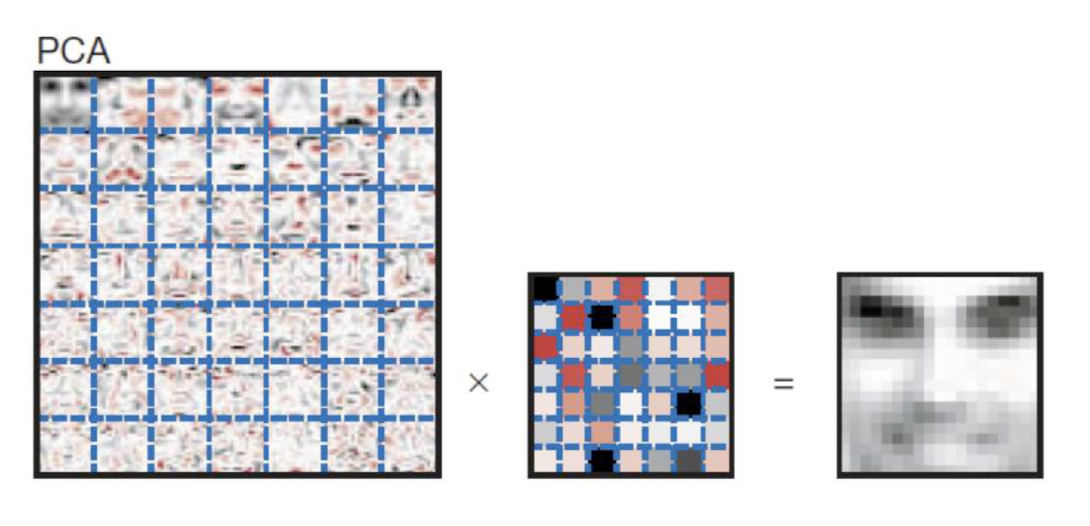
\includegraphics[width=\textwidth]{figures/pca_face}
    \caption{Factors identified by principal component analysis in a face reconstruction task.}
    \label{fig:pca}
\end{marginfigure}

The topic model introduced above is intimately related to matrix decomposition, where we see that
the topic variable $z \in [k]$ plays the role of a rank constraint. More specifically, we define
the following matrices, \[
    \mat{U} \doteq [p(w_j \mid z)] \in [0,1]^{m \times k}, \quad \mat{V} \doteq [p(z \mid d_i)] \in [0,1]^{n \times k}.
\]
We then form $\hat{\mat{N}} = \mat{U} \transpose{\mat{V}}$, which is a rank-$k$ matrix. We
interpret the entries of this new matrix $\hat{\mat{N}}$ as \[
    \hat{N}_{ji} = \transpose{\vec{u}_j} \vec{v}_i = \sum_{z=1}^{k} p(w_j \mid z) p(z \mid d_i) = p(w_j \mid d_i).
\]
Note that $\hat{\mat{N}}$ is a relative version of $\mat{N}$, where $N_{ij} \approx s_i
    \hat{N}_{ij}$. Thus, we have a matrix decomposition with additional constraints, \[
    u_{jz} \geq 0, \forall j \in [m], z \in [k], \quad v_{zi} \geq 0, \forall i \in [n], z \in [k].
\]
This is known as non-negative matrix factorization (NMF).\sidenote{For NMF, we can use the ALS
    algorithm, where we add projection steps to enforce non-negativity, \[
        u_{jz} = \max\{ 0, u_{jz} \}, \quad v_{zi} = \max \lft\{ 0, v_{zi} \rgt\}.
    \]
    \Cref{fig:nmf,fig:pca} show identified factors of NMF and PCA on a face reconstruction task.
    As can be seen, NMF tends to identify part-based representations and its features are sparse,
    because there is no way of removing added features, due to the non-negativity constraint. In
    other words, NMF models must be careful in what they add.} The objective follows from the maximum
likelihood principle, \[
    \ell(\mat{U}, \mat{V}; \mat{N}) = \sum_{i=1}^{n} \sum_{j=1}^{m} N_{ij} \log \hat{N}_{ij}, \quad \hat{\mat{N}} = \mat{U} \transpose{\mat{V}}.
\]
Further, we have normalization constraints on the row and column level, namely \[
    \sum_{j=1}^{m} u_{jz} = 1, \forall z \in [k], \quad \sum_{z=1}^{k} v_{zi} = 1, \forall i \in [n].
\]
Thus, we have a special case of non-negative matrix decomposition with a log-likelihood objective.

\subsection{Embeddings}

In natural language, the atomic units of meaning are symbols, such as words. Generally, these
symbols do not carry their meaning with them. Rather, their meaning come from their use within its
language. The idea of embeddings is to learn representations that capture semantics by embedding
symbols in vector space. Specifically, we want to learn a mapping from words to vectors such that
the vectors represent word semantics.

The latent variable approach to this problem is to learn latent representations that are predictive
of observations. Thus, we need to design a task such that the latent representations of the words
must have some form of semantics to be able to perform the task well. In the skip-gram model, we
use the task of predicting whether a word is in the context of another.\sidenote{Rupert Firth:
    ``You shall know a word by the company it keeps.''} Effectively, we are treating the embedding of
each word as a latent variable that predicts the co-occurring of context words. After the model has
converged, we do not care about performing the task well, but rather the parameters (embeddings) of
the model that lead to the task being performed well.

This task has the following likelihood function that we wish to maximize, \[
    \ell(\vec{\theta}; \vec{x}) = \sum_{t=1}^{T} \sum_{\delta \in \mathcal{I}} \log p(x_{t+\delta} \mid x_t; \vec{\theta}),
\]
where $\vec{\theta}$ contains the embeddings as parameters of this model and $\mathcal{I}$ is a set
of displacements, \eg, $\mathcal{I} = \{ -R, \ldots, -1, 1, \ldots, R \}$. The probabilities are
computed by normalized inner products, \[
    p(v \mid w; \vec{\theta}) = \frac{\exp \langle \vec{z}_w, \vec{z}_v \rangle}{\sum_{u \in \Sigma} \exp \langle \vec{z}_w, \vec{z}_u \rangle}.
\]
We can further refine this by introducing biases $b_v \in \R$ to explicitly control the marginal
probability and using different embeddings for conditioned and predicted words,\sidenote{This is
    necessary, because words are often not within their own context window, but will have a high inner
    product, because their vectors are equal.} leading to \[
    p(v \mid w; \vec{\theta}) = \frac{\exp(\langle \vec{\zeta}_w, \vec{z}_v \rangle + b_v)}{\sum_{u \in \Sigma} \exp(\langle \vec{\zeta}_w, \vec{z}_u \rangle + b_u)}
\]
with parameters \[
    \vec{\theta}_w = (\vec{z}_w, \vec{\zeta}_w, b_w) \in \R^{2m+1}.
\]
Sufficient statistics for this model is a co-occurrence matrix, where \[
    N_{vw} = | \{ t \mid x_t = w, x_{t+\delta}=v, \delta \in \mathcal{I} \} |.
\]
The log-likelihood can then be computed by \[
    \ell(\vec{\theta}; \vec{x}) = \sum_{v \in \Sigma} \sum_{w \in \Sigma} N_{vw} \lft( \langle \vec{\zeta}_w, \vec{z}_v \rangle + b_v - \log \sum_{u \in \Sigma} \exp (\langle \vec{\zeta}_w, \vec{z}_u \rangle + b_u) \rgt).
\]

The problem with this approach is that computing the normalization constant is expensive. We can
discard normalization by reformulating the prediction problem as a classification problem. For
this, we also need positive samples, \[
    \mathcal{S}^+ = [(x_t, x_{t+\delta}) \mid t \in [T], \delta \in \mathcal{I}]. \margintag{The $[]$ notation indicates a multiset.}
\]
And, additionally we need negative samples, which we randomly sample, \[
    \mathcal{S}^- = [(x_t, v_{tj}) \mid t \in [T], v_{tj} \sampleiid q, j \in [r]],
\]
where $q$ is a distribution over $\Sigma$ and $r$ is the sampling factor. Generally, $q$ is chosen
to satisfy \[
    q(w) \propto p(w)^{\alpha},
\]
where typically $\alpha = \nicefrac{3}{4}$. The intuition behind this is that what matters most in
learning semantic representations is not the very frequent words, which carry little meaning, and
also not the infrequent words, but the in-between range. This choice of $\alpha$ makes them more
likely to be sampled, as shown in \Cref{fig:alpha}.

\begin{marginfigure}
    \centering
    \begin{tikzpicture}
        \begin{axis}[
                width=\textwidth,
                height=\textwidth,
                xlabel=$p(w)$,
                ylabel={$p(w)^{\alpha}$},
                xmin=0, xmax=1,
                ymin=0, ymax=1,
            ]
            \addplot[samples=200,mark=none,domain=-0.5:1.5,thick,blue] {x^(0.75)};
            \addplot[samples=2,mark=none,dashed, domain=-0.5:1.5] {x};
        \end{axis}
    \end{tikzpicture}
    \caption{Plot of $p(w)^{\alpha}$ for $\alpha = \nicefrac{3}{4}$.}
    \label{fig:alpha}
\end{marginfigure}

We can then define a logistic log-likelihood function that we wish to minimize, \[
    \ell(\vec{\theta}, \vec{x}) = \sum_{(w,v) \in \mathcal{S}^+} \log \sigma(v, w; \vec{\theta}) + \sum_{(w,u) \in \mathcal{S}^-} \log (1 - \sigma(u, w; \vec{\theta})).
\]
This does not require computing a normalization constant.

\paragraph{Pointwise mutual information.}

Let $p(v,w)$ denote the true distribution of co-occurring words and by $q(v,w) = p(w)p(v)$ the
distribution used for negative sampling. The optimal Bayesian classifier would then be \[
    \mathbb{P}((v,w) = \mathrm{true}) = \frac{\pi p(v,w)}{\pi p(v,w) + (1-\pi) q(v,w)},
\]
where $\pi$ is the prior probability of a true pair. Considering the pre-image (logit) of the
logistic function, we get
\begin{align*}
    h^\star_{vw} & = \sigma^{-1} \lft( \frac{\pi p(v,w)}{\pi p(v,w) + (1-\pi) q(v,w)} \rgt)                                                                                                                         \\
                 & = \log \lft( \frac{\pi p(v,w)}{\pi p(v,w) + (1-\pi) q(v,w)} \cdot \frac{\pi p(v,w) + (1-\pi) q(v,w)}{(1-\pi) q(v,w)} \rgt) \margintag{$\sigma^{-1}(p) = \log \frac{p}{1-p}, \quad p \in (0,1)$.} \\
                 & = \log \lft( \frac{\pi p(v,w)}{(1-\pi) q(v,w)} \rgt)                                                                                                                                             \\
                 & = \log \frac{p(v,w)}{q(v,w)} + \log \frac{\pi}{1-\pi}.
\end{align*}
Hence, in the case of balanced classes $\pi = \nicefrac{1}{2}$ (equivalent to $r=1$) and $\alpha = 1$, we get \[
    h^\star_{vw} = \log \frac{p(v,w)}{p(w)p(v)},
\]
which is the pointwise mutual information.

\paragraph{GloVe.} Global word vectors (GloVe) considers word embedding models in terms of matrix factorization. It
maximizes a different objective, \[
    \ell(\vec{\theta}, \mat{N}) = \sum_{\substack{v,w \in \Sigma \\ N_{vw} > 0}} f(N_{vw}) \lft( \log N_{vw} - \log \hat{N}_{vw} \rgt)^2, \quad \hat{N}_{vw} = p(v,w; \vec{\theta}),
\]
which is a weighted square loss on the log-scale. In practice, the following weighting function is
used, \[
    f(N) = \min \lft\{ 1, \lft( \frac{N}{N_{\max}} \rgt)^{\alpha} \rgt\},
\]
where often $\alpha = \nicefrac{3}{4}$.

The idea of this objective is that the we can work with an unnormalized conditional probability
distribution and simply choose \[
    \log p(v,w) = \langle \vec{\zeta}_w, \vec{z}_v \rangle.
\]
The reason for this is that the squared objective is two-sided, whereas a likelihood objective will
always increase if we increase probabilities and the balancing effect comes purely from the
normalization.

GloVe can be interpreted as a low-rank matrix factorization with \[
    \mat{U} \doteq \transpose{[\vec{\zeta}_1, \ldots, \vec{\zeta}_n]}, \quad \mat{V} \doteq \transpose{[\vec{z}_1, \ldots, \vec{z}_n]}.
\]
Then, we have the following matrix of unnormalized probabilities, \[
    \log \hat{\mat{N}} = \mat{U} \transpose{\mat{V}}.
\]
The GloVe objective is a weighted Frobenius norm of the approximation residual between the observed
log-count matrix and a low-rank factorization of embedding matrices. As a special case, consider \[
    f(N) = \min \{ 1, N \},
\]
which results in a matrix completion problem,
\begin{align*}
    \mat{U}, \mat{V} \in \argmin_{\mat{U}, \mat{V}} & \sum_{i=1}^{n} \sum_{j=1}^{n} \mathbb{1}\{ N_{ij} > 0 \} \lft( \log N_{ij} - \lft( \mat{U} \transpose{\mat{V}} \rgt)_{ij} \rgt)                                                                                                             \\
                                                    & = \lft\| \Pi_{\mathbb{1}\{ \mat{N} > 0 \}} \lft( \log \mat{N} - \mat{U} \transpose{\mat{V}} \rgt) \rgt\|_F^2. \margintag{This is a matrix completion problem with $\mat{A} = \log \mat{N}$ and $\omega_{ij} = \mathbb{1}\{ N_{ij} > 0 \}$.}
\end{align*}

We can optimize $\mat{U}$ and $\mat{V}$ by stochastic gradient descent,
\begin{align*}
    \vec{\zeta}_w & \gets \vec{\zeta}_w + 2 \eta f(N_{vw}) (\log N_{vw} - \langle \vec{\zeta}_w, \vec{z}_v \rangle) \vec{z}_v  \\
    \vec{z}_v     & \gets \vec{z}_v + 2 \eta f(N_{vw}) (\log N_{vw} - \langle \vec{\zeta}_w, \vec{z}_v \rangle) \vec{\zeta}_w,
\end{align*}
where we sample $(v,w)$ at random.
